\chapter{Auswahl untersuchter Filterbauweisen}
\label{ch:auswahl}
Nach Aussage von Karsten Schulz von Freudenberg Filtration Technologies sind Verschleißerscheinungen in Tiefenfiltern nicht relevant. Auslegungs- und Konstruktionsfehler, z.B. beim Design der Strömungskanäle, ausgenommen, sind Tiefenfilter in aller Regel zugesetzt, bevor überhaupt mechanischer Verschleiß auftreten kann.
Im Gegensatz hierzu können Oberflächenfilter, welche mit einem Reinigungsmechanismus ausgestattet sind, durchaus mehrere Jahre in Betrieb sein und abhängig von Wartungsqualität und Belastung bis zu 10 Jahre funktionstüchtig sein. \cite{Schulz} 
Auslegungsfehler können allerdings genauso selbstverständlich auftreten, wie geänderte Rahmenbedingungen (z.B. geänderte Verkehrslage, Baustellen etc.), die eine vorherige Auslegungsrechnung ungültig machen. Es tritt in der Praxis also durchaus auch bei Tiefenfiltern Verschleiß und unvorhergesehene Schäden auf.\newline
Im Kontext dieser Arbeit sind zwei unterschiedliche Vorgehensweise in Bezug auf die beiden Filtertypen Tiefen- und Oberflächenfilter denkbar, welche in den folgenden Unterkapiteln vorgestellt werden.
\section{Filteranlagen mit Abreinigungsmechanismus}
Filteranlagen mit Abreinigungsmechanismus werden häufig bei größeren \ac{lta}'s eingesetzt. Beispiele hierfür wären große Lackierhallen, Produktionshallen, in denen faserverstärkte Werkstoffe bearbeitet werden, oder auch viele spanende Fertigungsverfahren eingesetzt werden. Diese Art von Filteranlagen sind nicht Teil der Arbeit, sollen an dieser Stelle der Vollständigkeit halber jedoch kurz vorgestellt werden, da sie ebenfalls Potenzial für eine KI-basierte Überwachung bieten. \newline
Auf Grund der relativ langen Standzeiten derartiger Filteranlagen ist eine umfangreichere Datenbasis verfügbar bzw. generierbar.
Auf Grund der Fahrweise dieser Anlagen mit abwechselnden Filtrier- und Abreinigungsphasen wäre der zunehmende Verschleiß z.B. an Hand des Vergleichs von erreichten Differenzdruckplateus zwischen Abreinigungsphasen denkbar (s. Abb. \ref{fi:druckverlust_abr}). 
\begin{figure}[H]
    \begin{center}
        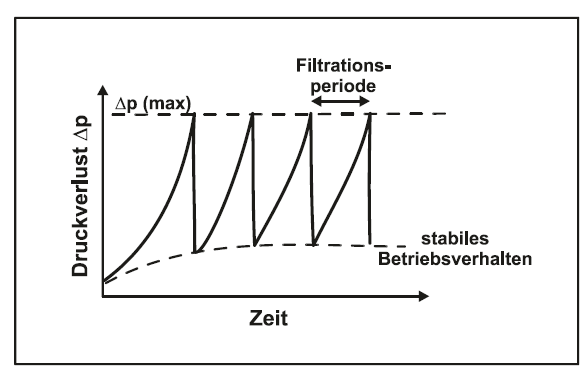
\includegraphics[width=0.55\textwidth]{images/druckverlust_wechsel.png}
        \caption[Druckverlust abreinigende Filter]{Verlauf des Druckverlustes bei Filtern mit Abreinigungsmechanismus \cite{immission} }
        \label{fi:druckverlust_abr}
    \end{center}
\end{figure}
Hieraus ließe sich mit aus Versuchen gewonnenen Daten leicht eine Verschleißkurve generieren, aus der dann Ausfallwahrscheinlichkeiten abgeleitet werden können. Da diese Filteranlagen in der Regel als ein Verbund aus Filterzellen ausgeführt sind, könnte man für die Versuche einzelne Zellen prüfen, was den Realisierungsaufwand reduzieren würde.
Außerdem ständen, im Gegensatz zu Tiefenfiltern, auch Daten aus der Abreinigungsphase zur Verfügung. Diese würden, bei entsprechender Abtastrate, einen guten Indikator für den Verschleißzustand des Filtermediums darstellen, da der Filterkuchen gegen Ende der Abreinigungsphase nahezu vollständig abgetragen wird. Im Filterbetrieb wäre es schwierig Aussagen über den Zustand des Filtermdiums zu treffen, denn der Filterkuchen trägt maßgeblich zur Bildung der Druckdifferenz und Filtrationsleistung bei, und kann somit mechanischen Verschleiß im eigentlichen Filter verschleiern.
\section{Filter zur Raumklimatisierung/lüftung}
In größeren Betriebsgebäuden, wie Bürogebäude, Schulen, Krankenhäuser etc. werden komplexe Lüftungsanlagen zur Klimatisierung und Lüftung eingesetzt. Ziel ist hierbei eine ausreichende Luftqualität und die Vermeidung von Schimmelbildung. Auch die Verbreitung von Keimen und Pilzsporen zu verhindern ist hierbei von Bedeutung, wie die Sars-CoV-2 Pandemie eindrücklich gezeigt hat.
Wie die Keimbelastung von Filtern in Gebäuden überwachbar bzw. vorhersagbar gemacht werden kann ist daher Gegenstand aktueller Forschung. Biologische Vorgänge wie Pilzwachstum oder Virenverbreitung mathematisch beschreibbar zu machen erfordert jedoch einen immensen Versuchsaufwand und die Arbeit eines interdisziplinären Forschungsteams, und soll daher nicht Teil dieser Arbeit sein.\newline
A priori sind vorallem in solchen Szenarien eingesetzte Vorfilter von anhaltender Luftfeuchte und anderen ungünstigen Wetterbedingungen betroffen. Hierbei kann sich die Feuchte in den Filtermedien niederschlagen, was bei einer Überwachung der Differenzdrücke als Überschreitung des Grenzwerts erkannt werden kann. In Konsequenz werden die Filter getauscht, obwohl diese eventuell im laufenden Betrieb getrocknet und im System belassen werden könnten. Die Fusion von Betriebs- und Umweltdaten, wie z.B. Wetterdaten, bietet daher ein vielversprechendes Konzept zur KI-basierten Überwachung solcher Anlagen.
\section{Auswahl anhand beispielhafter Anlage}
\label{sec:auswahl_konk}
Die Auswahl der behandelten Filter erfolgt an einer beispielhaften Klimazentrale (s. Abb. \ref{fi:beispielanlage}), welche aus der VDI3677-2 als typische Anlage übernommen wurde. Die konkrete Auswahl der Filter erfolgt auf Grundlage von Herstellerempfehlungen zur Verwendung der einzelnen Filterklassen. Die Bauweisen werden bei dieser beispielhaften Auswahl bewusst variiert, um anhand des Beispiels die typischen Bauweisen vorzustellen. Für die erste Filterstufe (s. 4 in Abb / Anhang: PSB/290 S) wird ein Grobstaubfilter G4 als Filtermatte verwendet, und dient als Vorfilter zum Schutz der nachgelagerten Systeme der Zuluftseite (unterer Abschnitt Abb. \ref{fi:beispielanlage}). Als zweite Filterstufe (s. 5 in Abb / Anhang: WinAir 90 8M), bzw. Endfilter vor der Verteilung an die Räume, wird ein Feinstaubfilter F7 in Taschenbauweise eingesetzt. Es ist nun üblich für Räume mit besonderen Anforderungen an die Luftqualität sog. endständige Filter in Form von Schwebstofffiltern einzusetzen. Hierfür wird (nicht in Abb. / Anhang: Viledon E11 610x610) im Beispielsystem ein Schwebstofffilter E10 in Kasettenbauweise eingesetzt. Nähere Angaben zu den Filtern in Bezug auf Verschleiß und Analyse der Datenblätter gewählter Filter erfolgt im Kapitel \ref{ch:Filterverschleiß}. Auf die Abluftseite des Systems wird nicht näher eingegangen, da mit dieser Auswahl bereits drei unterschiedliche Filter gemäß Aufgabenstellung \ref{ch: Aufgabenstellung} abgedeckt sind.\newpage
\begin{figure}[H]
    \begin{center}
        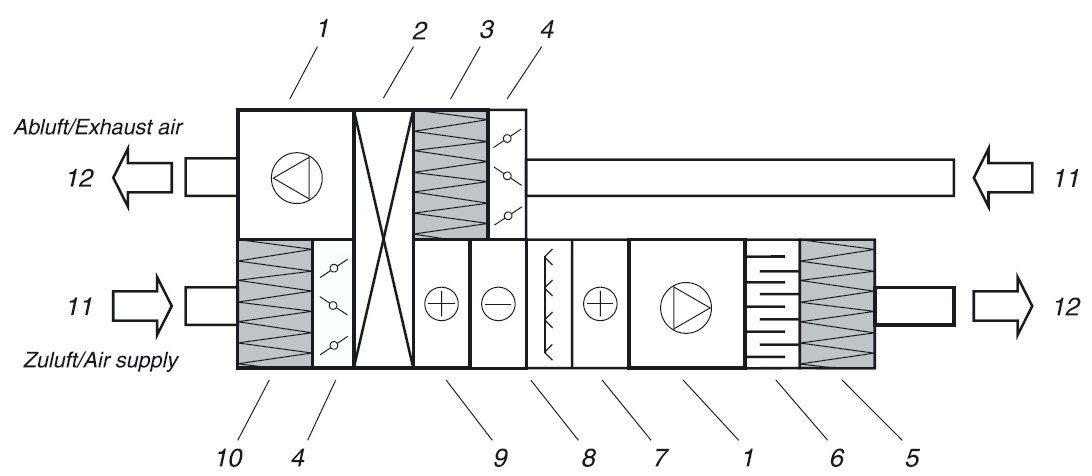
\includegraphics[width=\linewidth]{images/beispielanlage.png}
        \caption[Typische Klimazentrale]{Typischer Aufbau einer  Klimazentrale nach VDI3677-2 \cite{vdi3677_2} }
        \label{fi:beispielanlage}
    \end{center}
\end{figure}
\begin{itemize}
    \item 1 Ventilator
    \item 2 Wärmerückgewinnung
    \item 3 Abluftfilter
    \item 4 Volumenstromregelung
    \item 5 2. Filterstufe
    \item 6 Schalldämpfer
    \item 7 Erhitzer
    \item 8 Befeuchter
    \item 9 Erhitzer/Kühler
    \item 10 1. Filterstufe
    \item 11 Zuluft
    \item 12 Abluft
\end{itemize}




